\section{Model for Cloud Platforms}
\label{sec:modelcloud}
The iterative and model based approach optimized configuration parameters for resource utilization. As argued in Insight 1, 
resource utilization as an optimization function is appropriate with the resources saved can be used by other tasks. On SQL-on-Hadoop
machines, this is not true. Moreover, the memory given to a particular container is determined by the Memory/vCPU of the instance type 
and any variation from the ratio is sub-optimal. Therefore a new optimization function focused on cumulative is more appropriate for the cloud.
The optimization function is described in the next section.

On cloud platforms, it is important to recommend instance types along with configuration parameters. We extend Algorithm \ref{jobfit} to determine
the best instance type for a SQL query.

In the last section, we describe experimental results of these additions to the model.

\noindent\subsubsection*{Cumulative Time Optimization Function}
\label{subsubsec:cumulative_time}
The optimization function is 
$\mathcal{T} = \sum_{i=1}^{n} t_i$ where $n$ is number of containers and $t_i$ is execution time for $i^{th}$ container. 

\noindent\subsubsection*{Algorithm}

\begin{algorithm}
\caption{optimizeCost} \label{cost_optimize}
\begin{algorithmic}[1]
\footnotesize
\REQUIRE $\mathcal{P}$ is the job parameters (defined in \ref{table:job_params} ), Set $\mathcal{I} = {i_1, i_2, i_3, ...} $ set of instance configurations (defined in \ref{table:inst_conf}), Cost Metric Function $\mathcal{M}$
\ENSURE Returns optimized job parameter across all the instance configurations in $\mathcal{I}$.
\RETURN $\min_{\forall i \in \mathcal{I}} \mathcal{M}(fitJob(\mathcal{P}, i), i)$
\end{algorithmic}
\end{algorithm}

\noindent\subsubsection*{Results}

We evaluated new cost metric defined for cloud on our customer workload on SparkSQL. Note that we have run our experiments in our customer environment against their real world data set. Due to which we could not use the same queries used in earlier evaluation for previous cost metric. We ran our experiments on Amazon Web Services. Figure \ref{fig:modelbaseddollarresult} shows the reduction percent on absolute dollar cost of running 3 customer queries. Dollar cost is determined by the cost of running a particular AWS instance for cumulative time of running query as defined in Section \ref{subsubsec:cumulative_time}.

\begin{figure}[h]
	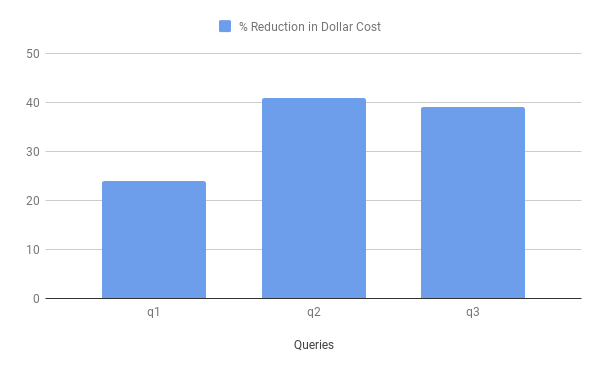
\includegraphics[width=\linewidth]{ModelExp.png}
	%\vspace*{-15pt}
	\caption{Model Based Result: Reduction percent in absolute dollar cost}
	\label{fig:modelbaseddollarresult}
\end{figure}
